\documentclass[norsk,a4,12pt,fleqn]{extarticle}
\usepackage[norsk]{babel} 
\usepackage[utf8]{inputenc} 
\usepackage{times}			% Default times font style
\usepackage[T1]{fontenc} 	% Font encoding \usepackage{amsmath} 		% Math package
\usepackage{mathtools} 		% Adds the declare paired 
							% delimeter command to make costom \abs and \norm
\usepackage{xfrac}			% Adds slanted fractions (sfrac)
\usepackage{cancel}			% Adds the cancel command, a slash through the symbol(s)
\usepackage{tabularx}		% Adds adjustable width on tabulars
							% environment.  
\usepackage{epstopdf}
\epstopdfsetup{update}
\usepackage{graphicx}
\usepackage{hyperref}
\usepackage[letterpaper, margin=0.6in]{geometry}
\usepackage{parskip}		% Norske avsnitt
\usepackage{siunitx}		% SI-enheter
\usepackage{tablefootnote}
\usepackage{tabularx}
\usepackage{listings}

% Alghorithm packages:
\usepackage{algorithm}
\usepackage[noend]{algpseudocode}

% Start custom \abs \norm 
\DeclarePairedDelimiter\abs{\lvert}{\rvert}%
\DeclarePairedDelimiter\norm{\lVert}{\rVert}%
% Swap the definition of \abs* and \norm*, so that \abs
% and \norm resizes the size of the brackets, and the 
% starred version does not.
\makeatletter
\let\oldabs\abs
\def\abs{\@ifstar{\oldabs}{\oldabs*}}
%
\let\oldnorm\norm
\def\norm{\@ifstar{\oldnorm}{\oldnorm*}}
\renewcommand{\ALG@name}{Algoritme}
\makeatother
% End custom \abs \norm 

\usepackage{titlesec}

% TODO: Put comments on this section*.
\newcommand{\eq}[1]{{\small\begin{align*}#1\end{align*}}}
\newcommand{\equ}[1]{{\small\begin{align}#1\end{align}}}
\newcommand{\mat}[1]{\begin{matrix}#1\end{matrix}}
\renewcommand\vec[1]{\mathbf{#1}}
\newcommand{\OP}[1]{\mathbf{\widehat{#1}}}
\newcommand{\op}[1]{\hat{#1}}
\newcommand{\unit}[1]{\mathbf{\hat{#1}}}
\renewcommand{\thesection}{\Roman{section}.}
\renewcommand{\thesubsection}{\Alph{subsection}.}
\renewcommand{\thesubsubsection}{\arabic{subsubsection}.}

\title{Prosjektoppgave i FYS2130, vår 2017 \\[1em]
    \Large Modellering av bølger på streng\\[2em]}
\author{Kandidatnummer: 15043} 

\begin{document}
\maketitle

I dette prosjektet er målet å simulere en vibrerende streng.

Jeg har jobbet sammen med kandidatnummer 15032.
Dette kan hovedsaklig sees på grafene.

\section*{Oppgave 1}

Vi bruker her ligningene (O.1), (O.2) og (O.3) fra oppgaveteksten til prosjektet.

Vi ønsker å utlede bevegelsesligningen for massepunktet 

Først tar vi utgangspunkt i likning (O.2) og løser for $y_i^+$. 
\begin{equation*}
    y_i^+ = \ddot{y_i}(\Delta t)^2 + 2 y_i^0 - y_i^- 
\end{equation*}

Fra ligning (O.3) har vi et uttrykk for kraften, dvs. akselerasjonen.
Dette setter vi inn i uttrykket over slik at
\begin{equation}\label{eq:yF}
    \ddot{y} = \frac{F_i}{m_i} \ \Rightarrow \ y_i^+ = \frac{F_i}{m_i}\Delta t^2 + 2y_y^0 - y_i^-
\end{equation}

Setter vi utrykket for \(F_i\) (ligning O.3) inn i likning ~\ref{eq:yF} 
får vi bevegelseslikningen vi er ute etter. 

\begin{equation}\label{eq:y}
    y_i^+ =  -(k_{i-1} + k_i)y_i^0 + k_{i-1}y_{i-1}^0 + k_iy_{i+1}\frac{(\Delta t)^2}{m_i} + 2y_y^0 - y_i^-
\end{equation}


Videre må vi se på hva slags endepunkter vi jobber med. Vi kan enten ha åpne 
eller reflekterende ender. 

Ved åpne ender setter vi kun inn kraften fra høyre i startpunkter og kraften fra venstre i endpunktet. 
Endepunktene vil dermed ha følgende form
\begin{equation*}
    y_0^+ =  -k_i(y_i - y_{i+1})\frac{(\Delta t)^2}{m_i} + 2y_y^0 - y_i^-
\end{equation*} 
\begin{equation*}
    y_{N-1}^+ =  -k_{i-1}(y_i - y_{i-1})\frac{(\Delta t)^2}{m_i} + 2y_y^0 - y_i^-
\end{equation*} 

Reflekterende ender får vi når verdien på svingning i endepunktet holdes på 0. 
Dette er det samme som en fast vegg, og vi kan gi endemassepunktene
en mye høyere masse sammenlignet med resten for å oppnå dette.

\section*{Oppgave 2}
Nå ønsker vi å utlede bølgeligningen for en vibrerende streng.
Vi introduserer en massetetthet, 
\begin{align}
    \mu = m/\Delta x, 
\end{align}
samt den konstante fjærstivheten
\begin{align} 
    \kappa = k\Delta x
\end{align}

Vi har at
\begin{equation*}
    F_i = m_i \frac{d^2y}{dt^2} = -(k_{i-1} + k_i)y_i^0 + k_{i-1}y_{i-1}^0 + k_iy_{i+1} 
\end{equation*}

Ved å sette inn for konstantene ender vi med

\begin{equation*}
    \frac{\kappa}{\mu} \left(\frac{y_{i+1}- 2y_i + y_{i-1}}{\Delta x^2}\right)
\end{equation*}

Inne i parentesen har vi den deriverte, \(\frac{d^2y}{dx^2}\).
Videre får vi
\begin{equation*}
    \frac{\kappa}{\mu} \frac{d^2y}{dx^2}
\end{equation*}. 

og får til slutt

\begin{equation*}
    \frac{d^2y}{dt^2} = v_B^2 \frac{d^y}{dx^2} 
\end{equation*}

\section*{Oppgave 3}
Vi har følgende betingelse på den 
numeriske hastigheten
\begin{align}
    \frac{\Delta x}{\Delta t} > v_B
\end{align}

Fra oppgave 2 har vi et utrykk for utbredelseshastigheten gitt ved
\begin{align}
    v_B = \sqrt{\frac{\kappa}{\mu}}
\end{align}
Innsatt i ligningen for den numeriske hastigheten får vi
\begin{align}
    \frac{\Delta x}{\Delta t} > \sqrt{\frac{\kappa}{\mu}} = \sqrt{\frac{k\Delta x^2}{m}}
\end{align}
Dermed blir en betingelse for tidssteget at
\begin{align}
    \Delta t < \sqrt{\frac{m}{k}}
\end{align}

Her ser vi at posisjonssteget $\Delta x$ er uavhengig av
$m$ og $k$. Det er ingen forflytting i $x$-aksen, og det eneste
$\Delta x$ gir er lengden på strengen, gitt antall massepunkter ($L=N\Delta x$).
Vi vil derfor bruke at $\Delta x = 1$.

I dette prosjektet vil vi fremover bruke at
\begin{align}
    \Delta t = 0.1\cdot \sqrt{\frac{m}{k}}
\end{align}

\section*{Oppgave 4}
Vi har nå alt verktøyet for å kunne regne på svingebevegelsen.
Startbetingelsen vår er
\begin{equation}
y_i^0 = \sin\left(7\pi \frac{i}{N-1}\right), \qquad 0\leq i \leq N-1
\end{equation}
Vi setter også denne verdien for det siste tidssteget, $y_i(t_{\text{max}})$.
Grunnen til dette er at vi trenger en god posisjon \textit{før}
vi begynner å telle. Siden Python regner element $-1$ som
det siste, slipper vi å legge inn en ekstra if-test for
startbetingelsene.
Denne verdien blir uansett overskrevet til slutt, og virker
kun som en «proxy» for $y_i(-\Delta t)$

Hadde vi valgt $y_i(-\Delta t) = 0$ ville det vært som om strengen
plutselig hoppet fra ro til en sinusbølge, som gir et annet resultat
enn det vi er interessert i.

Resultatet kan sees i figur \ref{fig:prob4}.
Vi ser her utbredelsen av en stående bølge.
Strengen vil altså bevege seg opp og ned på samme sted.

\begin{figure}[H]
    \label{fig:prob4}
    \centering % center the image horizontally
    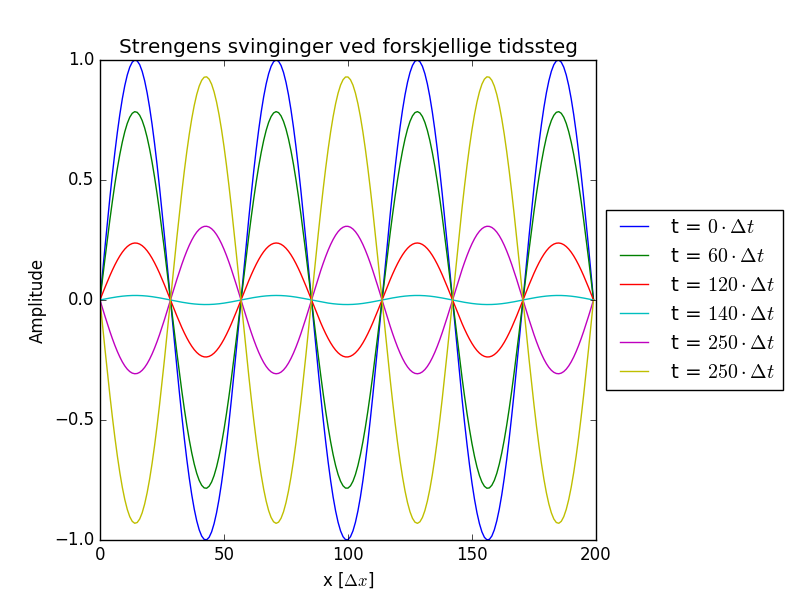
\includegraphics[width=0.7\textwidth]{../src/problem4.png}
    \caption{} 
\end{figure} 

\section*{Oppgave 5}
Målet vårt i denne oppgaven er 
å finne frekvensen
til strengens svingning
ved midtpunkt ($y_{99}(t)$)
ved å bruke tre 
forskjellige metoder:
en analytisk (forventet) verdi,
en numerisk verdi som vi
«teller» oss frem til.
og en verdi fra frekvensspektret
gitt ved Fourier-transformasjonen.
Selve bevegelsen kan sees i figur \ref{fig:prob5svingning}

Vi begynner med den «analytiske»
løsningen, og bruker denne
til å finne antall
tidssteg som trengs for ti perioder.

En bølge har egenskapen
at utbredelseshastigheten
er gitt ved
\begin{align}
    v_B = f\lambda
    \label{eq:vB2}
\end{align}

Bølgelengden $\lambda$
er gitt ved
bølgetallet $n$.
Vi kan se på $n$
som antall fysiske topper
strengen har når den vibrerer.
Fra initialbetingelsen
$\sin\left(7\pi \frac{i}{N-1} \right)$
ser vi at vi må ha
bølgetallet $n = \frac{7\pi}{2\pi} = 3.5$.
Siden strengen er $N$
punkter lang, kan vi finne
bølgelengden ved
\begin{align}
    \lambda = \frac{N}{n} =
    \frac{200}{3.5}
\end{align}
i vårt tilfelle.

Nå kan vi regne ut den analytiske
frekvensen
\begin{align}
    f_{analytisk} = \frac{v_B}{\lambda} = 0.391311896062 \text{ Hz}
\end{align}

Denne frekvensen gir oss mulighet
til å regne ut antall tidssteg
for ti perioder.
\begin{align}
    \text{\#tidssteg} =
    \frac{10}{\Delta t\cdot f}
    \sim 5715
\end{align}
når vi runder opp.

Videre vil vi regne frekvensen
numerisk  ved
å telle hvor mange perioder vi
har i et tidsrom.
Jeg gjorde dette ved å 
velge startpunktet til
funskjonen, $y_{99}(t_0 = 0) = -1$,
og sjekke hvor mange ganger
den oppnådde denne verdien.
Deretter regnet jeg ut frekvensen
ved 
\begin{align}
    f_{numerisk} = 
    \frac{\text{\#tellinger}}
    {\Delta t(t_1-t_0)}
    = 0.393120249209 \text{ Hz}
\end{align}

En annen måte for å regne ut den numeriske
frekvensen hadde vært å sjekke hvor ofte
funksjonen byttet fortegn.
Denne ville vært mer generell, da
jeg har som utgangspunkt at den første
$y$-verdien er $-1$.


Til slutt ser vi på 
frekvensspektret til
funksjonen gjennom
å Fourier-transformere signalet.
Resultatet kan sees i
figur \ref{fig:prob5fourier}.
Verdien i toppunktet
er
\begin{align}
    f_{fourier} = 0.391331462636
    \text{ H Hz}
\end{align}

\begin{figure}[H]
    \label{fig:prob5svingning}
    \centering % center the image horizontally
    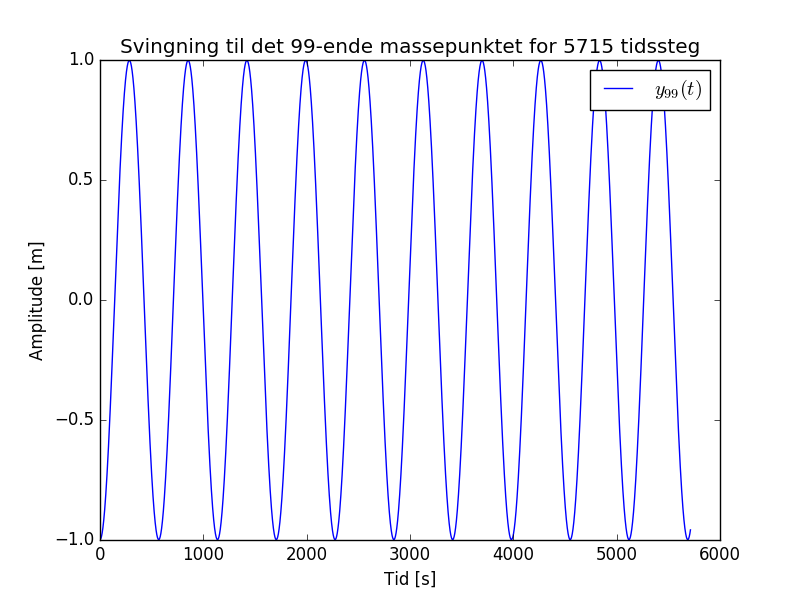
\includegraphics[width=0.7\textwidth]{../src/problem5-svingning.png}
    \caption{} 
\end{figure} 

\begin{figure}[H]
    \label{fig:prob5fourier}
    \centering % center the image horizontally
    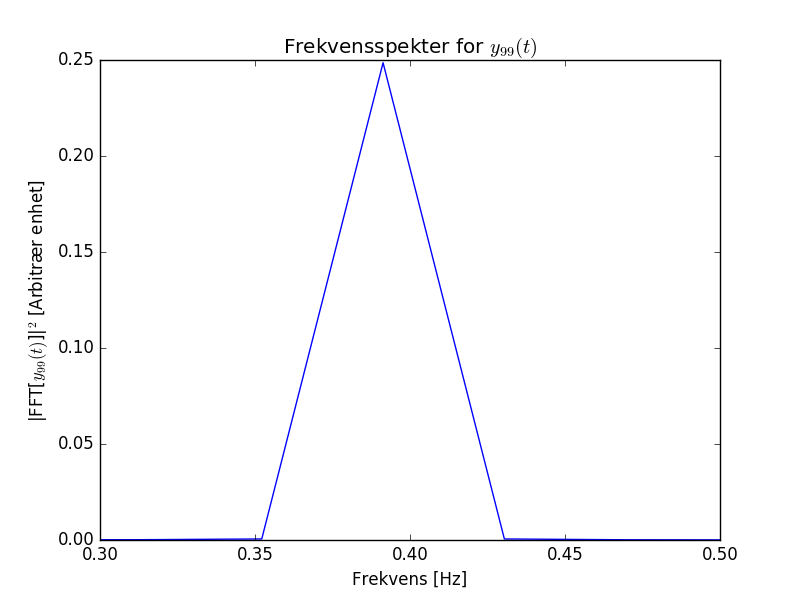
\includegraphics[width=0.7\textwidth]{../src/problem5-frekvens.png}
    \caption{} 
\end{figure} 

\section*{Oppgave 6}
For å regne ut energien
til hele strengen ved ett
tidssteg, må vi summere
kinetisk og potensiell
energi over alle $i$-verdier.

For en fjær er kinetisk energi gitt ved
\begin{align}
    E_k = \frac{1}{2}\sum_i m_i v_i^2
\end{align}
og potensiell energi ved
\begin{align}
    E_p = \frac{1}{2}\sum_i k_i \Delta y^2
\end{align}

For strengen tilsvarer det at
$\delta y = y_{i+1} - y_i$.
Hastigheten $v_i$ har vi ikke et
uttrykk for, men siden vi har
diskretisert strengen, kan vi
regne ut denne numerisk ved
\begin{align}
    v_i^0 = \frac{y_i^+ - y_i^0}{\Delta t}
\end{align}

Vi har plottet resultatet i figur
\ref{fig:prob6}.

Her ser vi at vi har en svingning
i energi, men den er relativt
liten. Det vil si at energien
er tilnærmet konservert, men
siden vi regner diskretisert
er det naturlig å forvente
små svinginger.

\begin{figure}[H]
    \label{fig:prob6}
    \centering % center the image horizontally
    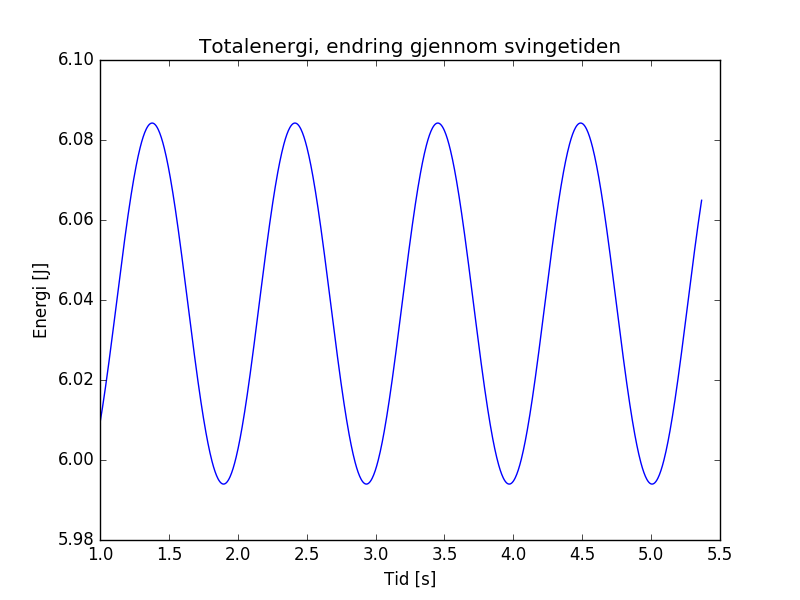
\includegraphics[width=0.7\textwidth]{../src/problem6.png}
    \caption{} 
\end{figure} 

\section*{Oppgave 7}
Vi vil nå se på en bølge formet
som en trekant.
Den vil ha følgende initialbetingelser
\begin{align}
    y_i^0 = y_i^- =
    \begin{cases}
        (i-69)/30\;\;\;70\leq i\leq 99\\
        (129-i)/30\;\;\; 100\leq i \leq 128\\
        0\;\;\; \text{else}
    \end{cases}
\end{align}

Ved å bruke programmet vi utviklet
i oppgave 4 og endre initialbetingelsene
til det ovenfor, får vi bevegelsen
i figur \ref{fig:prob7}.

Her ser vi at bølgen deler seg i to
og beveger seg i hver sin retning,
hver med halvparten av amplituden til
den original bølgen.
Når bølgene treffer sine respektive
vegger vil reflekteres ned på undersiden
av strengen. Deretter møtes de igjen
og blir en stor bølge med
den original amplituden.

Når vi setter initialbetingelsene
til å være slik at $y_i^0 = y_i^-$,
altså at startbetingelsen og
posisjonen før er like, vil det
være det samme som at vi har en superposisjon
av to mindre bølger som beveger seg i hver sin retning.
Dermed vil bølgen dele seg i to i de
neste tidsstegene og gå i hver sin retning.

\begin{figure}[H]
    \label{fig:prob7}
    \centering % center the image horizontally
    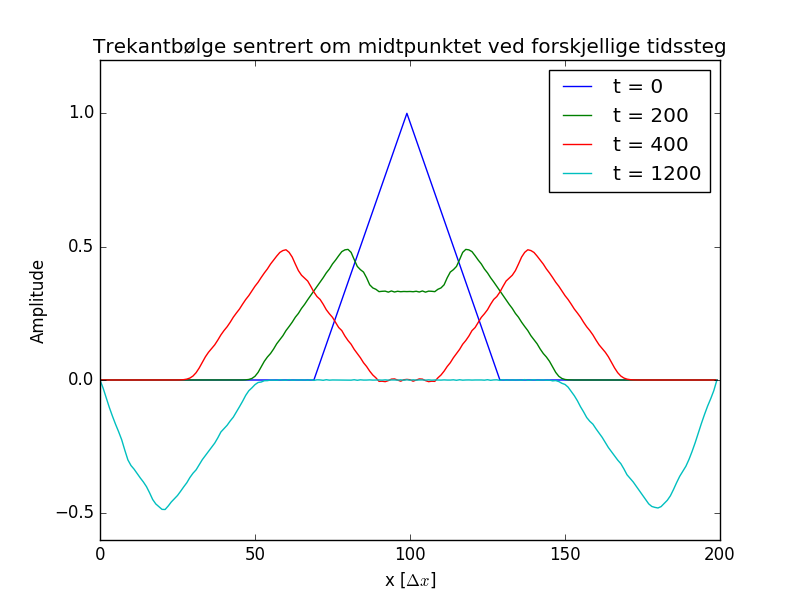
\includegraphics[width=0.7\textwidth]{../src/problem7.png}
    \caption{} 
\end{figure} 


\section*{Oppgave 8}
Vi sentrerer nå strengen rundt indeks $i=30$, slik
\begin{equation}
y_i^0 =
\begin{cases}
\frac{i}{30} & 1 \leq i \leq 30\\
\frac{60-i}{30} & 31 \leq i \leq 60\\
0 & \text{else}
\end{cases}
\end{equation}

Deretter vil vi at trekanten skal bevege seg mot høyre.
Det gjør vi det å legge til pre-initialbetingelsen
\begin{equation}
y_i^- =
\begin{cases}
y_i^0+\Delta t\cdot v_B/30 & 0 \leq i \leq 29\\
y_i^0-\Delta t\cdot v_B/30 & 30 \leq i \leq 59\\
0 & \text{else}
\end{cases}
\end{equation}

Dette er for å gi verdien i det forrige tidssteget
som endringen av det som ville vært før om bølgen hadde kommet fra venstre.
Se figur \ref{fig:prob8}.

\begin{figure}[H]
    \label{fig:prob8}
    \centering % center the image horizontally
    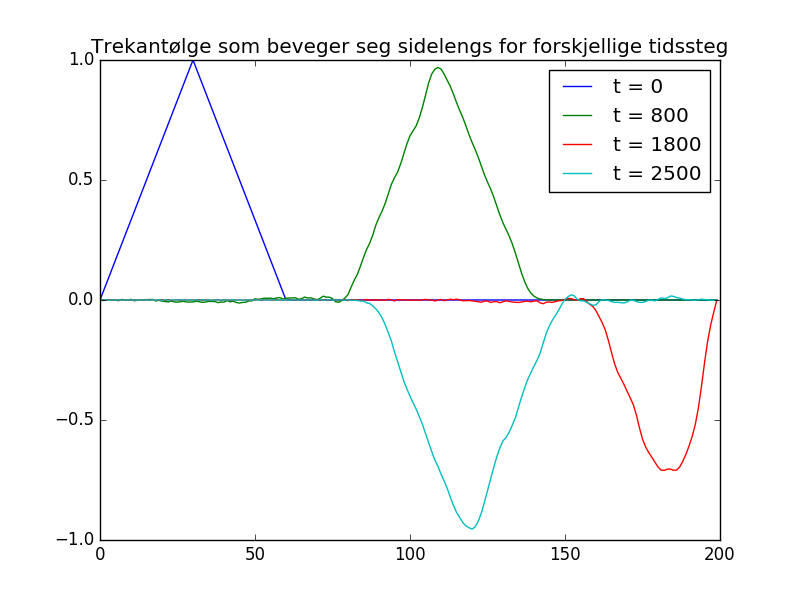
\includegraphics[width=0.7\textwidth]{../src/problem8.png}
    \caption{} 
\end{figure} 

\section*{Oppgave 9}

Nå lager vi tråden 200 punkter lenger
og gjør disse massepunktene tre ganger så tunge.
Vi sender fortsatt bølgen til høyre, men
nå vil deler av den bli reflektert tilbake,
mens resten vil gå over i den tykkere enden av
tråden. Se figur \ref{fig:prob9}.

Vi får at transmittert bølge har amplitude
\begin{align}
    T \sim 0.693
\end{align}
og reflektert bølge har amplitude
\begin{align}
    R \sim -0.259
\end{align}

Vi kan regne ut forholdet i impedans som
\begin{align}
    \frac{z_1}{z_0} = \sqrt{\frac{{3mk}}{mk}} = \sqrt{3} \sim 1.732
\end{align}

De følgende relasjonene gjelder for
reflesjons- og transmisjonsamplitudene
\begin{align}
    R = \frac{z_0 - z_1}{z_0 + z_1}
\end{align}    
\begin{align}
    T = \frac{2z_0}{z_0 + z_1}
\end{align}

Det gir oss følgende forhold for
den reflekterte bølgen
\begin{align}
    \frac{z_1}{z_0} = \frac{1-R}{1+R} \sim 1.699
\end{align}
    
og følgende for den transmitterte 
\begin{align}
    \frac{z_1}{z_0} = \frac{2}{T} - 1 \sim 1.886
\end{align}

Som vi ser av dette ligger verdiene våre ganske
nærme opptil den teoretiske verdien.
Fordi vi gjør disse utregningene diskret og
numerisk vil det alltid være litt støy.
Som vi ser av figur \ref{fig:prob9} beveger
ikke bølgen seg som en perfekt trekant.
Dermed kan vi ikke forvente at den teoretiske
verdien vil stemme perfekt overens med våre.
\begin{figure}[H]
    \label{fig:prob9}
    \centering % center the image horizontally
    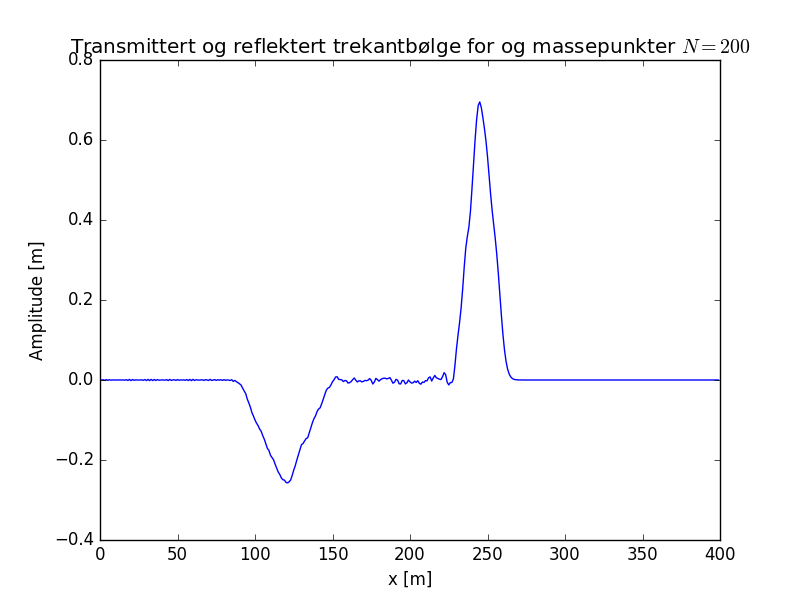
\includegraphics[width=0.7\textwidth]{../src/problem9.png}
    \caption{} 
\end{figure} 


\section*{Appendiks – kodesnutter}
Dette er programmene som er brukt for å kjøre koden som lager plottene over.
Noen steder vil det være mulig å kommentere inn visse deler for
å se animasjoner av bølgebevegelsene.
\subsection*{Oppgave 4}
\lstinputlisting[language=python, title = Svingebevegelse]{../src/problem4.py}
\newpage
\subsection*{Oppgave 5}
\lstinputlisting[language=python, title = Frekvensspekter]{../src/problem5.py}
\newpage
\subsection*{Oppgave 6}
\lstinputlisting[language=python, title = Energikonservering]{../src/problem6.py}
\newpage
\subsection*{Oppgave 7}
\lstinputlisting[language=python, title = Trekant på streng]{../src/problem7.py}
\newpage
\subsection*{Oppgave 8} 
\lstinputlisting[language=python, title = Trekant som beveger seg]{../src/problem8.py}
\newpage
\subsection*{Oppgave 9} 
\lstinputlisting[language=python, title = Trekant på tykkere streng]{../src/problem9.py}

\end{document}
